\chapter{State of the Art}

Physically based rendering is the process of generating synthetic images indistinguishable from the perception of the real world. These images are generated according to a geometric model of the scene and models for every material and light source present. With this information is possible to simulate the light transport process from the light sources to the camera through the scene in order to synthesize an image. With this simulation, the radiance for each pixel of the image is determined, being radiance the radiant power incident on a given region per area and solid angle unit.

\todo[inline]{Intro on heterogeneous systems}

\section{Path Tracing}

One of the first solutions to the global ilumination was introduced by \cite{Kajiya} when he defined the problem of rendering as the resolution of an integral equation, also know as the rendering equation.

\begin{equation}
I(x,x')=g(x,x')\left[e(x,x')+\int_{S}^{} \rho(x,x',x'')I(x',x'')dx''\right]
\label{eq:render_eq}
\end{equation}

Where:

\begin{tabular}{r l}
$I(x,x')$ & is related to the intensity of light passing from point $x$ to $x'$ \\
$g(x,x')$ & is the geometric term \\
$e(x,x')$ & is related to the intensity of emited light from $x$ to $x'$ \\
$\rho(x,x',x'')$ & is related to the intensity of light scattered from $x''$ to $x$ through $x'$\\
\end{tabular}
\\

This equation translates to how much light arrives at a given point from a given direction. This integral equation can not be calculated analitically, so its expected value is calculated through Monte Carlo Integration. Based on this, the goal is to trace a light transport path, with points $x_0$ .. $x_n$ in which $x_0$ is a point on a light source and $x_n$ is a point on the camera lens. 
Commonly, these paths are traced from the camera to the light source, to ensure that paths sampled fall in the image plane and to capture reflection and refraction paths. However caustic paths have a very low sampling probability, reaching zero if using point light sources. Tracing paths form the light source to the camera however sample caustics more effectively but specular paths can not be sampled.

\begin{figure}[H]
\centering
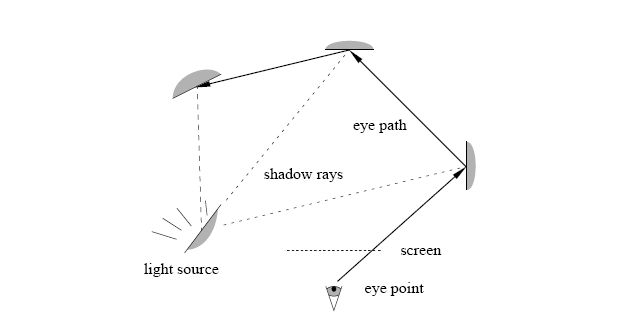
\includegraphics[width=0.75\linewidth]{img/ptDiagram.jpeg}
\caption{\label{img:ptdiag} Path Tracing Algorithm}
\end{figure}

\section{Bidirectional Path Tracing}

\gls{bdpt}, proposed independently by \cite{Veach} and \cite{Lafortune} combines both forward and backwards path tracing in one single method that can become more robust than the previous two alone. Although with a different mathematical background, both authors propose that the method should sample pairs of sub-paths containing a light sub-path and a camera sub-path. Then, each vertex of one sub-path is explicitly connected to all vertices of the other one, generating a new set of light transport paths.

\begin{figure}[H]
\centering
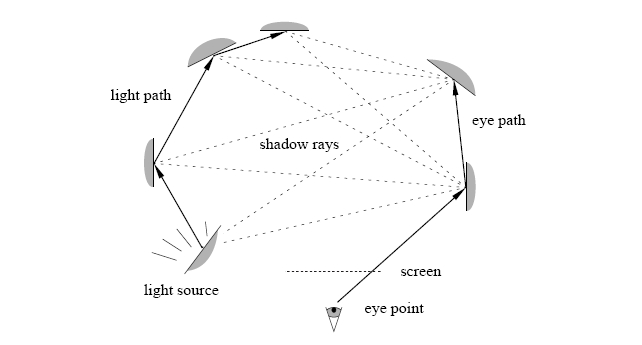
\includegraphics[width=0.75\linewidth]{img/bptDiagram.jpeg}
\caption{\label{img:bptdiag} Bidirectional Path Tracing Algorithm}
\end{figure}

In order to make the algorithm more robust, \cite{Veach} proposed the Path Space Integration Framework and \gls{mis}. The first consists in converting the problem of light transport from a recursive integral equation (~\ref{eq:render_eq}) to a simple integral over the space of all light transport paths.
\begin{equation}
I_j=\int_\Omega f_j(x)d\mu (x)
\label{eq:path_int}
\end{equation}
where $\Omega$ is the set of all light transport paths of all lenghts, $\mu$ is a measure on this space of paths and $f_j$ is the measurement contribution function.

Multiple Importance Sampling is a technique that attempts to combine multiple sampling techniques in a probably good way in order to minimize variance.
\begin{equation}
F = \sum_{i=1}^n \frac{1}{n_i} \sum_{j=1}^{n_i} \omega_i (X_{i,j}) \frac{f(X_{i,j})}{p_i (X_{i,j})}
\label{eq:mis}
\end{equation}
Being $n$ the number of sampling techniques and $n_i$ the number of samples for technique $i$, this estimator attributes a weight $\omega$ to each sample. The balance heuristic is a simple and robust way to calculate these weights and is demonstrated that no other heuristic is much better \citep[p.~264]{Veach}.
\begin{equation}
\omega_i (x) = \frac{n_i p_i (x)}{\sum _k n_k p_k (x)}
\label{eq:balance}
\end{equation}
In order to use \gls{mis} in Bidirectional Path Tracing one must consider that each path of a given length can be sampled in several ways: a path of lengh $n$ can be sampled by using whatever light and camera sub-paths of $s$ and $t$ vertices as long as $n=s+t+1$. Given this it is just needed to apply the heuristic above to calculate the respective weight for that path.

\begin{equation}
I=\sum_{s \geq 0}\sum_{t \geq 0}\omega_{s,t}(x_{s,t})\frac{f_j (x_{s,t})}{p_{s,t}(x_{s,t})}
\label{eq:bpt}
\end{equation}

This algorithm is much more robust than path tracing, as it can sample many light transport paths efficiently and robustly. Nonetheless, this algorithm is not perfect for every situation, as it has dificulty sampling reflected caustics \citep{Georgiev}.

%\section{Metropolis Light Trasport}

%In an effort to improve the efficiency of light transport algorithms, \cite{Veach} proposed the adaptation of the Metropolis Sampling algorithm to the light trasport problem. This algorithms starts from one point in the function domain and generates a random walk such that in the limit, the sampling distribution is proportional to the function value, called the stationary distribution function. These new samples however, may not allways be accepted, and have an acceptance probability given by equation ~\ref{eq:acc_prob}.
%\begin{equation}
%a(x\xrightarrow{}y) = min \left\{ 1 , \frac{f(y)T(y\xrightarrow{}x)}{f(x)T(x\xrightarrow{}y)} \right\}
%\label{eq:acc_prob}
%\end{equation}
%where $a(x\xrightarrow{}y)$ is the acceptance probability from state $x$ to $y$ and $T$ is the the transition probability for the mutation being applied. As in the limit, the samples are distributed proportionaly to the function value, all samples have the same contribution to the final result.

%Applying this algorithm to the light transport problem, the function domain is the space of light transport paths and the function value is the contribution these paths have in the final image. The \gls{mlt} algorithm starts by generating a light transport path, using \gls{bdpt} for instance, and then aply mutations to that path using the acceptance probability defined in ~\ref{eq:acc_prob}.

%As the initial sample in the algorithm was not sampled according to the stationary distribution function, the algorithm exhibits startup bias, because only in the limit the samples converge to stationary distribution function and until then the results may be heavly influenced by the choice of the initial path. This problem is solved by sampling a set of paths, assigning each a weight $W_0 = f(X_0)/p_0 (X_0)$, and then select a subset of these paths with a probability proportional to these weights. Then, all these paths are assigned the same weight that is the average of all previously sampled weights. This solves two problems: removes start-up bias and calculates the normalization weight of the samples, scaling them to the right value.

%An important part of this algorithm are the mutations. In his work, \cite{Veach} proposed a set of mutations that aimed to solve some well known problem of light transpor algorithms, namely reflected caustics. However, \cite{Kelemen} proposed a simpler and robust form of mutation in the primary sampling space. Instead of trying to directly mutate the paths, mutations would be applied to the pseudo-random numbers used to generate them, being this perturbation smaller the higher the contribution of the sample in order to keep the acceptance probability high. One important property of the mutaions used in the Metropolis algorithm is that these must be able to transit from any point in the function domain to any other possible point, or else the algorithm would not respect the principle of ergodicity. In order to do that, sometimes it is needed to perform a large step mutation, that is regenerate all the random numbers used.

\section{Photon Mapping}

The previous algorithms attempted to solve the problem of global illumination by sampling light transport paths from the light source to the camera. \gls{pm} however, attempts to calculate the radiance at any given point by estimating a photon density \citep{Jensen}.

In a first phase the algorithm traces packets of photons from the light sources into the scene and stores them in a range search acceleration structure, the photon map. In a second phase, rays are traced from the camera and the photon map is consulted to calculate the photon density in the neighborhood of the hitpoints. One technique used to reduce the variance of this algorithm is the use of distinct photon maps for caustics and diffuse indirect ilumination and consult these maps differently: the caustics map is accessed directly while for diffuse ilumination a final gathering step is performed. In final gathering, rays are traced from the hit points into the scene and in the intersections of these rays the diffuse map is consulted.

\begin{figure}[H]
\centering
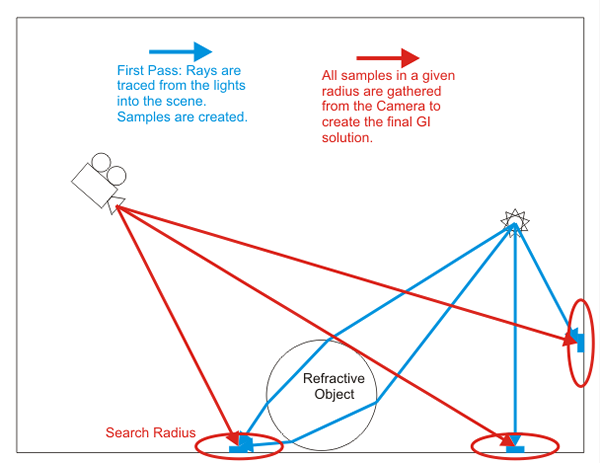
\includegraphics[width=0.75\linewidth]{img/pmDiagram.png}
\caption{\label{img:pmdiag} Photon Mapping Algorithm}
\end{figure}

This algorithm, unlike all the previously mentioned algorithms, introduces bias, because there is an aproximation of the photon map search area to an infinitly small area. This causes the algorithm to not converge to the correct result but to an aproximation with an unknown error (bias).

Although biased, this algorithm performs well in the handling of caustics, even reflected and refracted caustics. However, the convergence rate for the overall diffuse ilumination is smaller than that of Bidirectional Path Tracing \citep{Georgiev}. Another backdraw of this algorithm is memory usage, since the more photons used to rendering, the larger the photon map has to be.

\subsection{Progressive Photon Mapping}

Photon Mapping is a biased algorithm, although if the number of photons used tends to infinity and the search radius in the photon map tends to zero, the bias is zero in the limit. This makes the bias in the algorithm consistent and this property can be used to improve the quality of the algorithm.

Instead of storing the positions of photons in the photon map, the hitpoints from the camera rays are stored in an acceleration structure. Then, when photons are traced from the light sources, a range search looks for any hitpoint in the neighborhood and the contribution of that photon is added to the corresponding pixels. In each iteration of the algorithm the search radius is decreased according to a constant parameter of the algorithm \citep{Hachisuka}.

\begin{figure}[H]
\centering
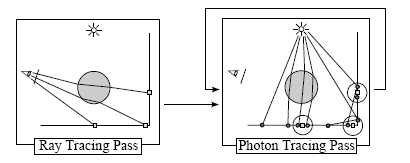
\includegraphics[width=0.75\linewidth]{img/ppmDiagram.png}
\caption{\label{img:ppmdiag} Progressive Photon Mapping Algorithm}
\end{figure}

This alteration to the algorithm improves the efficiency of Photon Mapping, namely in terms of memory usage, now fixed proportionaly to the size of the image, instead of proportional to the number of photons used. Although with Progressive Photon Mapping the bias may be zero in the limit, this algorithm also produces more useless work the longer it runs, since as the search radius decreases with the execution, more photons are traced that do not contribute to the final image.

\subsection{Bidirectional Photon Mapping}

In order to increase the robustness of the Photon Mapping technique, \cite{Vorba} proposed the \gls{bpm} algorithm. Instead of using a heuristic to determine the use of final gather and direct photon map consult, this algorithm uses \gls{mis} in order to increase the robustness of the algorithm, mostly when glossy materials are present.

This algorithm operates mostly like \gls{pm} but using only one photon map. In the rendering phase, instead of tracing only primary rays, a whole path is traced, and at every intersection of this path the photon map is consulted. During this step every photon contribution is independently weighted according to the probability it was generated.

This algorithm can also be progressive by reducing the search radius of the photon map at each iteration.

\section{Vertex Connection and Merging}

This new algorithm proposed by \cite{Georgiev}, combines two complementary algorithms in order to create a more robust rendering algorithm. As seen previously, Bidirectional Path Tracing has high convergence rate and can handle most types of ilumination effects, however it has problem rendering reflected or refracted caustics. On the other hand, the family of Photon Mapping algorithms has no problem dealing with caustics but has an overall low convergence rate. The combination of these two algorithms into a new one, Vertex Connection and Merging, through \gls{mis} is much more robust than the original algorithms alone.

The combination of Photon Mapping and Bidirectional Path Tracing required the reformulation of one of these algorithms, since they calculate the image values through different mathematical frameworks: while Bidirectional Path Tracing calculates an integral on the path space, Photon Mapping calculates a photon density estimation. To achieve this, Photon Mapping was reformulated as a path sampling technique, where a path is successfully sampled if the last vertex of the light sub-path falls into the search area of a vertex from the camera sub-path. These two vertices are effectively merged so the last vertex in the light sub-path is not considered part of the generated path itself but only as a conditional test of the acceptance of this new path. For this new path sampling technique, called Vertex Merging, an associated probability density function is needed to use multiple importance sampling. 
\begin{equation}
p_{VM}=[\pi r^2 p(x_{s-1}\xrightarrow{}x_{s}^{*})]p_{VC}(x)
\label{eq:pvm}
\end{equation}
where $p_{VC}(x)$ is the probability of generating path $x$ through Bidirectional Path Tracing and the initial part is the probability density funcion for the last light sub-path vertex to intersect the merging area of the last camera sub-path vertex.

\begin{figure}[H]
\centering
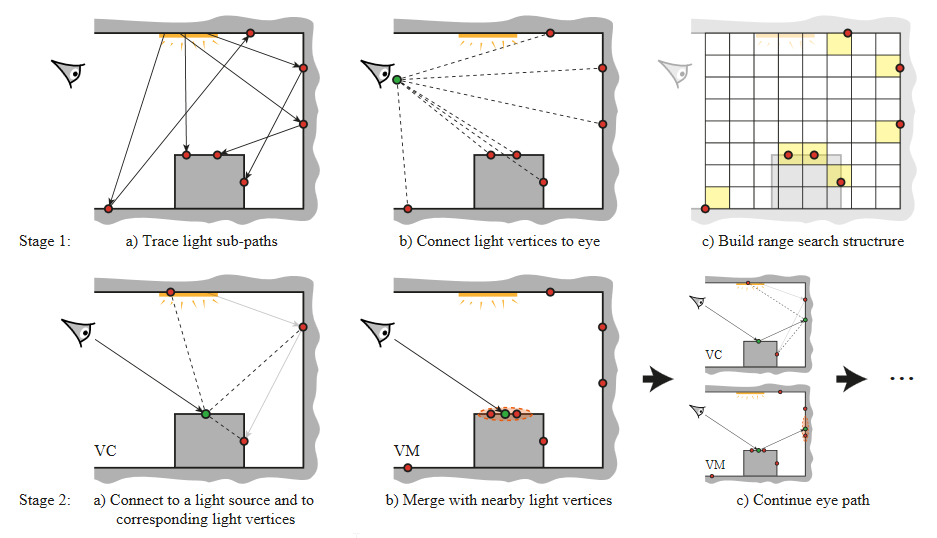
\includegraphics[width=\linewidth]{img/vcmDiagram.png}
\caption{\label{img:vcmdiag} Vertex Connection and Merging Algorithm}
\end{figure}

With a new path sampling technique, Vertex Merging, in conjunction with Bidirection Path Tracing, or Vertex Connection, it is possible to combine these two techinques using \gls{mis} to achieve robustness. This new combined algorithm starts like Bidirectional Path Tracing by tracing a set of paths from the light sources, and stores the vertices in a range search acceleration structure. Then when the camera sub-paths are being traced, each vertex of the camera sub-path is connected to all the vertices of the respective light sub-path, and searches the acceleration structure for any vertices from any light sub-path viable for merging.

This combined light transport algorithm maintains the high convergence rate of Bidirectional Path Tracing, while being able to handle caustics efficiently like Photon Mapping. The efficiency of this algorithm can still be improved by applying \gls{mcmc} techniques on top of it \citep{Georgiev}.

\section{Heterogeneous Systems}

An heterogeneous system is a computing system with different processing devices with different architectures. Indeed, most average computers are heterogeneous systems that contain a multi-core \gls{cpu} used for most tasks and a massivelly parallel \gls{gpu} used mainly for graphics rasterization. These two processors have separate addressing spaces, communication between them is costly, and even the programming model is different between them. This imposes difficulties to developers and inhibits portability of the code across diferent platforms \citep{Kunzman}. However there are potential performance gains in using both devices since there is additional computational power available. 

\subsection{DICE}

Developing applications for heterogeneous platforms is a difficult task as explained previously. DICE \citep{Barbosa} is an application framework for developing heterogeneous applications that aims to ease the process of development for heterogeneous platforms containing both \gls{cpu} and \gls{gpu}, with an emphasis on irregular workloads.

%DICE uses a task model in which tasks are scheduled by the system throughout the various available processors. The workload is distributed by generating sub-tasks of finer granularity and assigning them to different processors. The main features of DICE are an adaptative scheduler that analyses the execution time of each submited task and uses that information to perform load balancing operations, and a memory manager that simplifies different addressing spaces by presenting the developer only one address space and transparently preforming copies between different addressing spaces whenever required \citep{Barbosa}.

DICE uses a task driven model that schedules work across processing devices through a granularity refinement. When a task is submited to the scheduler, sub-tasks of finer granularity are generated and executed on the available devices. This scheduler analises the execution time of the task on each device to enhance the workload distribution in order to attain maximum performance. DICE also provides memory manager that abstracts different addressing spaces by presenting the developer only one address space and transparently performing copies between different addressing spaces whenever required.

DICE tasks support a variety of execution modes. The developer can provide a single kernel and the task can execute automatically on \gls{cpu} and \gls{gpu}, while it is also possible to provide the task with specialized code for each arquitecture. The specialized \gls{gpu} implementation can be provided as a CUDA kernel or as a call to specialized libraries. These possibilities allow a simple programming model while retaining the possibility of refinement, arquitechture specific optimizations and the use of external optimized libraries.

\subsection{StarPU}

%\todo[inline]{talk about starPU concurrent work}

%StarPU is a framework that provides high-level programming abstractions, integrated data management and enhanced scheduling mechanisms. It also provides an unified execution model working together with dynamic scheduling policies. The run-time features a data management system that entails several features: automatic work decomposition and data transfers, communication and computation overlapping, data pre-getching and locality aware scheduling, among others. StarPU has davanced data management and sophisticated scheduling techniques, such as the Heterogeneous Earliest Finish Time approach.

StarPU \citep{augonnet2011starpu} is an framework whose goal is similar to DICE. It amis to provide high level abstractions of an heterogeneous system, providing data management facilities and enhanced scheduling mechanisms, such as the Heterogeneous Earliest Finish Time approach. The data management system provides features such as automatic work decomposition, transparent data transfers between devices, communication and computation overlapping data pre-fetching and locality aware scheduling, among others.